\chapter{Oxygen Reduction in \Nm{}}
\label{chap:oxygenreduction}
\section{Aerobic Reduction of Oxygen}
\subsection{Introduction}
The first dataset I used in my iterative approach to parameter estimation was of a simple oxygen reduction experiment carried out in aerobic conditions. This dataset is the simplest biologically as under aerobic conditions and without the presence of any microaerobic substrates (nitrite or nitric oxide) the only respiratory pathway that is active is the oxygen reducing one. Additionally, the other parts of a respiratory chain influence the oxygen reducing pathway either by competing for electrons, or chemically inhibiting it. The relevant portions of the electron transport chain are shown graphically in Figure \ref{fig:o2_resp_chain}.

\begin{figure}[tbp]
	\centering
	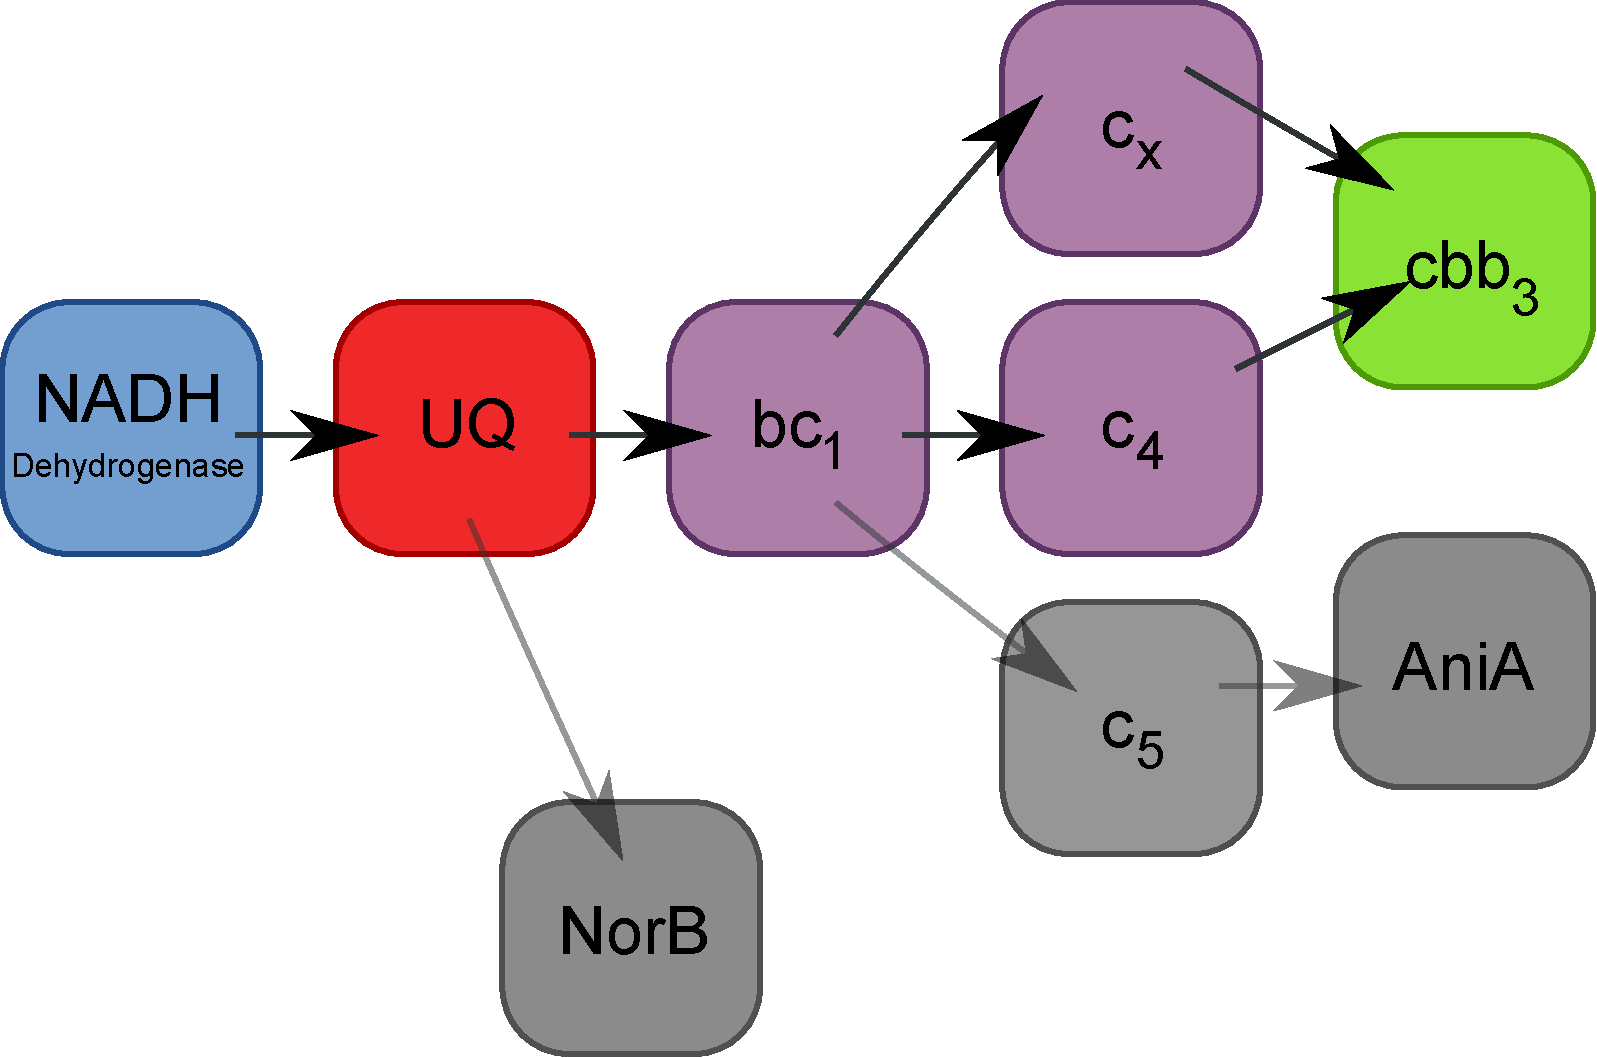
\includegraphics[width=14cm]{05-oxygenreduction/data/o2_resp_chain.pdf}
	\caption[Oxygen reducing electron transport chain of \Nm{}]{{\bf Oxygen reducing electron transport chain of \Nm{}.} This shows the complete electron transport chain of \Nsm{} with the components irrelevant to oxygen reduction greyed out. In the mathematical model all of the purple elements (cytochromes) are amalgamated into one entity.
	\label{fig:o2_resp_chain}}
\end{figure}

The equations that describe this portion of the electron transport chain are:
\begin{eqnarray*}
\frac{d[O_2]}{dt} & = & \beta(1-[O_2]/K_O) - k_{1}[C_a][O_2]\\
\frac{d[Q_a]}{dt} & = & g([Q] - [Q_a]) - l_3[Q_a]([B] - [B_a]) - f[Q_a]([X]-[E])\\
\frac{d[E]}{dt} & = & -k_3([C] - [C_a] - [C_X])[E]  - m_3([A] - [A_a])[E] + f[Q_a]([X]-[E])\\
\frac{d[C_a]}{dt} & = & k_3([C] - [C_a] - [C_X])[E] - k_{1}[C_a][O_2] - k_5[C_a][NO]
\end{eqnarray*}
These equations describe the change in concentration of oxygen over time, which is the experimentally observable value, the reduction state of the quinone pool and the reduction state of the cytochrome ``pool''. This portion of the model involved 13 parameters and variables which I tried to estimate (the model actually contains 17 such parameters and variables, but under these conditions the remaining 4 are set to 0 as they are related to nitrite reduction effects).

\subsection{Results}

Modelling oxygen reduction was the simplest both experimentally and mathematically. MC58 cultures were grown in aerobic conditions for around 3 hours, or until the $\mathrm{OD}_{600}$ had reached 0.3-0.9. Cultures were then transferred to the electrode chamber and the oxygen concentration was recorded as the culture respired. Once the culture had become anaerobic it was re-aerated by bubbling air through the culture with a sterile pasteur pipette. This  restored oxygen levels throughout the culture and they began respiring oxygen once more.

The experiments used to generate data for oxygen reduction are highly repeatable and consistently generate the same basic result of a linear reduction of oxygen with time.

The final solved output of the parameter estimation for this dataset can be seen in Figure \ref{fig:o2sim}. 
\subsubsection{Generation of Prior Probability Distributions}
In accordance with the integrative scheme I introduced in Chapter \ref{chap:paramest}, I attempted to estimate the distributions of the parameters involved in modelling these data. In order to do this I needed to create probability distributions to act as priors to feed into the estimation system as I am using a Bayesian approach. These probability distributions were generated from data obtained in the published literature, which is described in Chapter \ref{chap:model}, and preliminary experimental data. I assumed that all the prior probabilities would be normally distributed, therefore the distributions I used were created under the following scheme:
\begin{itemize}
	\item Where the literature value had bounds associated with it (i.e. published with $\pm{}$ values), I assumed that the bounds covered $3 \sigma$ of the normal distribution. This essentially assumes that 99.7\% of the distribution falls within the given bounds.
	\item Where the literature value has no bounds associated with it (i.e. published as a single figure), I assumed that a range of $\pm 10\%$ was covered by $3 \sigma$ of the normal distribution. This means that 99.7\% of the distribution falls within $\pm 10\%$ of the given value.
	\item Where there are no literature values available, the value was estimated based on preliminary experimental data and no bounds were associated. In this case the prior was free to be perturbed giving it an effective range of $0 < x < \infty$.
\end{itemize}
With reference to the above, the initial probability distributions used to start the Monte-Carlo run are shown in Figure \ref{fig:oxypriors}. As can be seen, very little information is readily available in the literature to populate the model.

\begin{figure}[tbp]
 \centering
 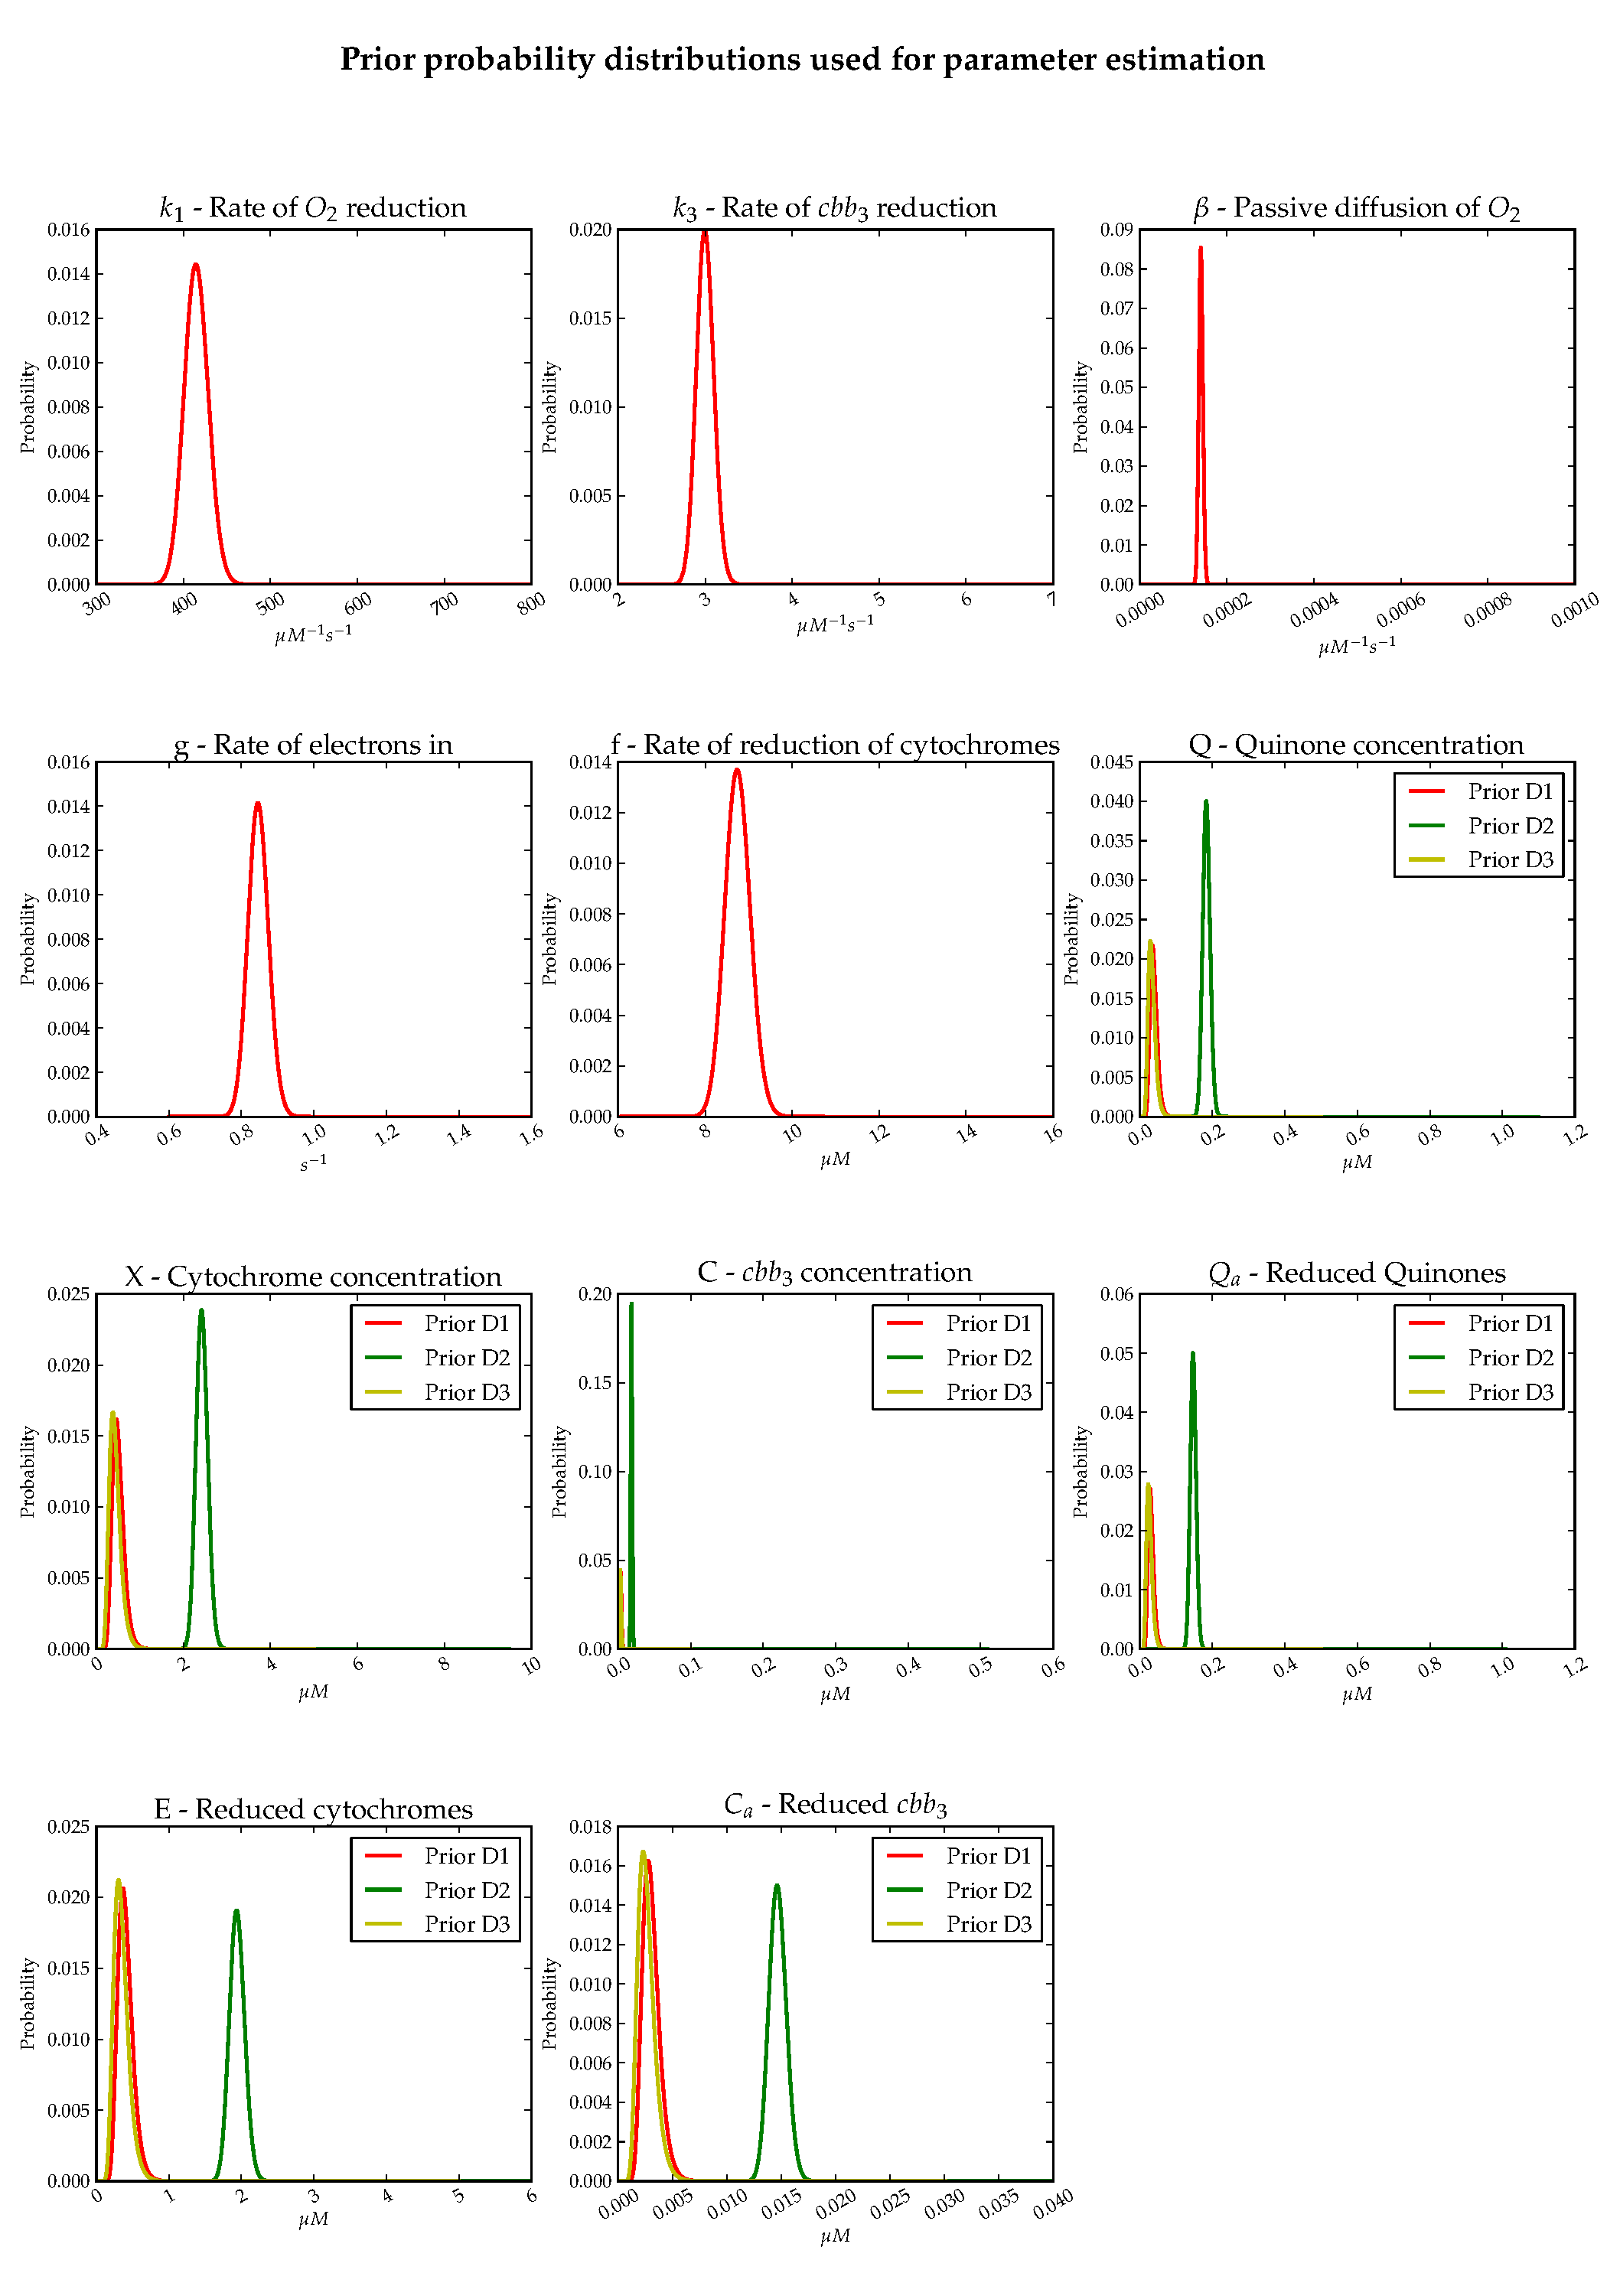
\includegraphics[width=15cm]{./05-oxygenreduction/data/priors.pdf}
 % priors.pdf: 1008x1008 pixel, 72dpi, 35.56x35.56 cm, bb=0 0 1008 1008
 \caption[Prior probability distributions for oxygen reduction]{{\bf Prior probability distributions for oxygen reduction}. These are the probability distributions used as priors by the parameter estimation algorithm. Where no values were available in the literature, the probability distribution represents a flat prior from 0 to $\infty$ with the initial value being determined by preliminary experiment.
 \label{fig:oxypriors}}
\end{figure}


\begin{figure}[tbp]
 \centering
 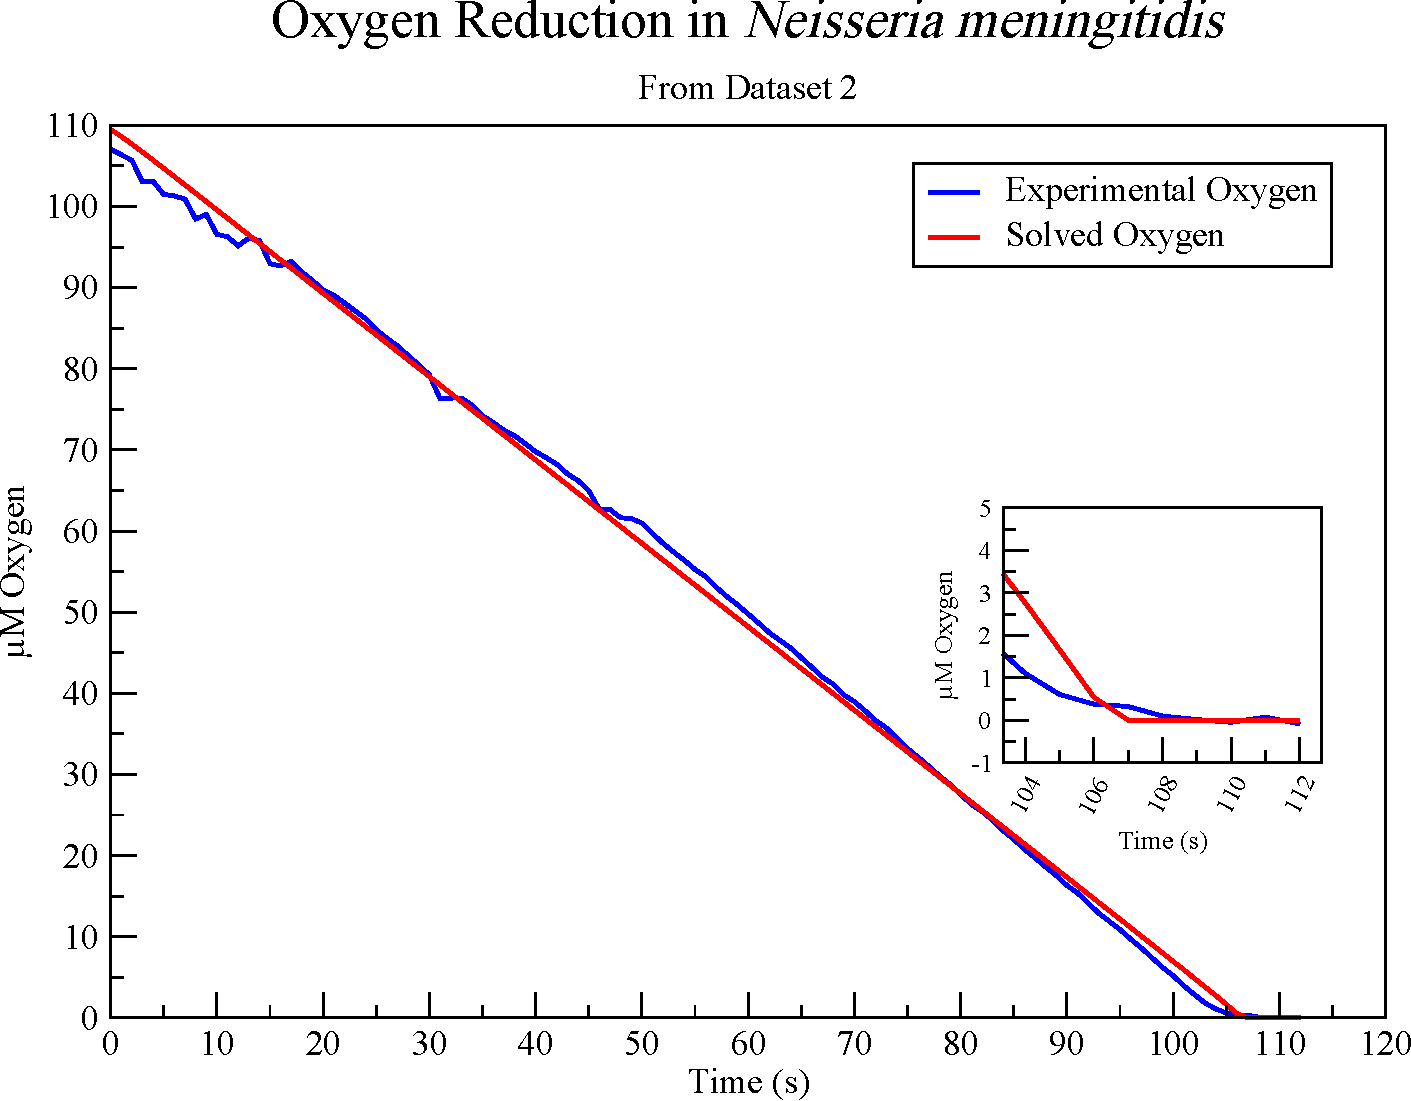
\includegraphics[width=14cm]{./05-oxygenreduction/data/o2sim.pdf}
 % o2sim.eps: 0x0 pixel, 300dpi, 0.00x0.00 cm, bb=0 0 794 595
 \caption[{Oxygen Reduction in \textit{Neisseria meningitidis}.}]{{\bf Oxygen Reduction in \textit{Neisseria meningitidis}.} This dataset shows the simple linear reduction of Oxygen in aerobic conditions. The high affinity of $\mathrm{cbb}_3$ for oxygen is evidenced by very little non-linearity at low oxygen concentrations. The solved output is a representative result of the parameter estimation system.
 \label{fig:o2sim}}
\end{figure}

\subsection{Discussion}
The experimental dataset shows that oxygen reduction in \textit{Neisseria meningitidis} is a simple linear system with the reductase having a high affinity for oxygen demonstrated by the almost complete lack of non-linearity as oxygen concentration approaches zero. This apparent simple linearity could be modelled with a high degree of accuracy with just 2 parameters in a simple $y=-mx+c$ system. However this does mean that the posterior distributions generated are very wide and therefore allows much greater freedom for the next dataset to explore the parameter space.

Given our knowledge of the underlying transport chain and the affinity of \cbbthree{} for oxygen, we expect a linear reduction of oxygen with high affinity over nearly two orders of magnitude. It is however remarkable that we can model this behaviour with so few components in the model, as it requires significant changes in the reduction state of the enzymes to achieve this.

\subsubsection{Analysis of Convergence}
\subsubsection{Analysis of Covariance}

\subsubsection{Rate of oxygen diffusion}